\documentclass[a4paper]{article}
\usepackage{amsmath}
\usepackage{amssymb}
\usepackage{subcaption} %for images 

% Packages
\usepackage{geometry}
\geometry{left=1.5cm, right=1.5cm, top=2.54cm, bottom=2.54cm}
\usepackage{graphicx, hyperref, setspace, titlesec, fancyhdr, multicol, parskip, indentfirst, etoolbox, caption, cite, xcolor, booktabs}
\newtheorem{theorem}{Theorem}

% Title Formatting
\titleformat{\section}{\centering\large\scshape}{\thesection}{1em}{}
\titleformat{\subsection}{\normalsize\bfseries}{\thesubsection.}{1em}{}

% Document Title
\title{
    \textbf{Using Prime Modulo Classes to Improve the HAR-RV Model} 
}
\author{}

\date{March 15, 2025}

% Section Numbering
% Define numbering format
\renewcommand{\thesection}{\Roman{section}.}
\renewcommand{\thesubsection}{\textit{\Alph{subsection}.}}
\renewcommand{\thesubsubsection}{\textit{\arabic{subsubsection}.}}

% Make titles italic as well

\titleformat{\subsection}{\normalfont\large\itshape}{\thesubsection}{1em}{}
\titleformat{\subsubsection}{\normalfont\itshape}{\thesubsubsection}{1em}{}


\setcounter{page}{5}

% Fancy Header Configuration
\pagestyle{fancy}
\fancyhf{} % Clear all header/footer fields
\setlength{\headheight}{17pt}

% First Page Header
\fancypagestyle{firstpage}{
    \fancyhf{}
    \fancyhead[C]{\textbf{Wat Street}}
}

% Default Header for Other Pages
\fancyhead[C]{\textbf{Wat Street}}
\begin{document}

\maketitle
\vspace{0.5cm}
\thispagestyle{firstpage}

% Authors Block
\begin{multicols}{3}
	\centering
	\textbf{Reshi Adavan}\\
	\textit{University of Waterloo}\\
	\textit{Wat Street}\\
	
	\vfill

   \textbf{Jacob Yan}\\
	\textit{University of Waterloo}\\
	\textit{Wat Street}\\
	
    \vfill

    \columnbreak

   \textbf{Kamakshi Sarvananthan}\\
	\textit{University of Waterloo}\\
	\textit{Wat Street}\\

     \vfill

    \textbf{Harman Singh}\\
        \textit{University of Waterloo}\\
        \textit{Wat Street}\\

    


    \columnbreak
	
    \vfill

 \textbf{Krish Modi}\\
	\textit{University of Waterloo}\\
	\textit{Wat Street}\\
	
    \vfill

    \columnbreak

\end{multicols}

\singlespacing
\setlength{\parskip}{6pt}
\setlength{\parindent}{0.5cm}

\begin{multicols}{2}
\setlength{\columnsep}{0.5cm}

\section{Introduction}
\vspace{0.3cm}
\noindent
Volatility plays a key role in financial market forecasting, particularly in the pricing of derivatives and risk management. A well-established model for predicting volatility based on historical data is the Heterogeneous Autoregressive model of Realized Volatility (HAR-RV) \cite{corsi2009}. This model leverages realized volatility, meaning volatility observed from historical high-frequency data, and incorporates information from multiple time horizons, typically daily, weekly, and monthly, to capture the persistence and heterogeneity of volatility dynamics. Although the HAR-RV model was originally developed for daily volatility forecasting, the same multi-horizon idea is useful in high-frequency settings where asset prices update on the order of seconds or minutes. The realized volatility over a given evaluation period is computed as:
\[
RV_t = \sqrt{\sum_{j=1}^n \left(\log\left(\frac{X_j}{X_{j-1}}\right)\right)^2},
\]
where $X_j$ denotes the asset price at the $j$-th intraday interval in that period.
\vspace{0.3cm}
\\ The standard HAR-RV forecast can be written as $$RV_{t+1} = C + \beta_d RV_t + \beta_wRVW_t + \beta_m RVM_t + \overline{\omega}_t,$$ where $\beta_d, \beta_w, \beta_m$ are learned parameters, $\overline{\omega}_t$ is the error term, $C$ is a constant, and $$RVW_t = \frac15\left(\sum_{i=1}^5 RV_{t-i+1}\right)$$ and $$RVM_t = \frac1{22}\left(\sum_{i=1}^{22} RV_{t-i+1}\right).$$ These terms represent weekly and monthly averages of realized volatility in terms of the shorter-horizon series. The goal of this paper is to present an order-aware extension of HAR-RV by adding learned features built from equivalence classes of prime moduli.
\vspace{0.3cm}
\\ The standard HAR-RV aggregation creates a symmetry problem. If two lagged realized-volatility values are swapped within the weekly average or within the monthly average, the corresponding HAR-RV features are unchanged, even though the order of volatility events can carry market information. We therefore add features such that, for any two of $RV_t, RV_{t-1}, \cdots, RV_{t-n+1}$ for a fixed horizon $n$, a swap can change at least one model input while holding the learned parameters fixed.
\section{Prime Modulo Classes}
\noindent To address this symmetry issue, we propose introducing additional terms that ensure any pair-wise swap of volatility values affects the model's predictions. Our goal is to find a minimal set of additional terms that captures these temporal dependencies while keeping the model parsimonious. The solution should generalize beyond the standard weekly and monthly intervals to arbitrary time periods, without compromising the model's predictive accuracy.
\vspace{0.3cm}
\\ First, we formulate our problem as follows: We would like to find a set of sets $\{a_j\}_{j=1}^c$ such that for all pairs $(x, y) \in \{1, 2, \cdots, n\}, x \neq y$, where $n$ is fixed, there exists some set $a_j$ such that $x$ is in $a_j$ but $y$ is not in $a_j$. We would also like to minimize $c$ for computational efficiency. The intuition is that each $RV_{t-i+1}$ for $1 \leq i \leq n$ corresponds to an element in $\{1, 2, \cdots, n\}$, so a swap between two $RV_{t-i-1}$'s would lead to a change in $RV_{t+1}$, if we reformulate the HAR-RV model as the following extended model: $$RV_{t+1} = C + \sum_{j = 1}^c\left(\beta_j \cdot \frac{1}{|a_j|} \sum_{i \in a_j} RV_{t-i+1}\right) + \overline{\omega}_t.$$ To reflect the HAR-RV model, we use $a_1 = \{1\}$, $a_2 = \{1, 2, 3, 4, 5\}$, and $a_3 = \{1, 2, \cdots, 22\}$.
\vspace{0.3cm}
\\ Intuitively, we let $a_j = \{1, 2, \cdots, j\}$ for all $j$. We consider consecutive windows starting from the current time; hence, it solves our volatility-swap symmetry problem while preserving the statistical and financial nature of the HAR-RV model. To prove this, consider any arbitrary pair $(x, y) \in \{1, 2, \cdots, n\}, x \neq y$. Without loss of generality, let $x<y$. Then, $a_x$ contains $x$ but not $y$, as desired. Now, can we optimize this exhaustive assignment? The answer is yes, we can.
\vspace{0.3cm}
\\ Given time horizon $n\in \mathbb{Z}^+$, we split $\{1, 2, \cdots, n\}$ into equivalence classes $$\{a_j\} = \bigcup_{i} \{[t]_{k_i}: 0 \leq t \leq k_i-1\}$$ for possibly multiple values of $k_i$ such that all $k_i$ are pairwise co-prime and $\displaystyle\prod_i k_i \geq n$.  In layman's terms, find the smallest number $N$ that's greater than our time horizon $n$, where $N$ is a product of the first consecutive distinct primes. Then, for each prime $p$ that divides $N$, we create sets based on equivalence classes in modulo $p$.
\begin{theorem}
    Considering the above construction, for any $(x, y) \in \{1, 2, \cdots, n\}, x\neq y$, there exists some $a_j$ such that $x \in a_j, y \notin a_j$.
\end{theorem}
\noindent \textbf{Proof: }Let $(x, y) \in \{1, 2, \cdots, n\}$ be arbitrary with $x \neq y$. Assume for the sake of contradiction that for all sets $a_j$ that contain $x$, they also contain $y$. Then, $$x \equiv y \pmod{k_i}$$ for all $k_i$. Since all $k_i$ are pairwise coprime, then by the Chinese Remainder Theorem, we get that $$x \equiv y \left(\text{mod }\displaystyle\prod_i k_i\right),$$ and letting $$k := \displaystyle\prod_i k_i,$$we get that $k | (x-y)$. Since $k \geq n$, and $$|x-y| \leq n-1 < k,$$ this implies that $|x-y| = 0$, so $x=y$, which is a contradiction. Therefore, this construction works.
\begin{flushright}
  $\square$
\end{flushright}
\vspace{0.3cm}
\noindent It remains to find $\{k_i\}$ that minimizes $c$, the number of extra terms we add. We formulate this as an optimization problem:
\vspace{0.3cm}
\begin{align*}
    (\star) & \text{ } \min_{t, k_i} \displaystyle\sum_{i=1}^t k_i \text{ }(= c)
    \\ \text{s.t.} & \text{ }\prod_{i=1}^t k_i \geq n
    \\ &\text{ $k_i$ pairwise coprime}.
\end{align*}
\vspace{0.3cm}
\begin{theorem}
    Let $c^*$ denote the optimal objective function in $(\star)$ and let $t^*$ be the optimal $t$ in this optimizer. Let $c$ be the sum of the first $t^{\star\star}$ primes where $t^{\star\star}$ is minimal such that $$N := \displaystyle\prod_{i=1}^{t^{\star\star}} p_i \geq n,$$where $p_i$ denotes the $i-$th prime. Then, $$c = c^* \cdot \frac{\log(n)}{\log(\log(n))}(1+o(1)).$$
\end{theorem}
\vspace{0.3cm}
\noindent The proof is omitted, but the main intuition is that using powers of repeated primes gives poor tradeoffs between the product constraint and the sum objective. Distinct small primes provide much better coverage per added feature while preserving the pairwise separation property above.
\vspace{0.3cm}
\\ The empirical section tests two prime-based extensions against the HAR-RV baseline. Prime Modulo (PM) uses the modular equivalence classes described above. Contiguous Prime (CP) keeps the same prime-motivated capacity but uses contiguous prime-length structure, preserving more local ordering information. The main draft focuses on HAR-RV, PM, and CP only. Additional supported variants and randomized controls are reserved for the ablation subsection once the aligned robustness run is complete.

\end{multicols}


\section{Results and Analysis}
\captionsetup{font=small,labelfont=bf,labelsep=period,hypcap=false}

\noindent
This section evaluates the baseline HAR-RV specification against the Prime Modulo (PM) and Contiguous Prime (CP) extensions on the ten-asset intraday panel used throughout the empirical study. The main text focuses on the 5-minute horizon. Unless otherwise noted, each reported metric is first computed asset by asset and is then summarized by the cross-sectional mean with a standard error across AAPL, AMZN, GOOGL, SPY, QQQ, EEM, FXI, GLD, HYG, and TLT.

\subsection{Overall Accuracy}

{\renewcommand{\thetable}{1A}
\begin{center}
\captionof{table}{Overall forecasting performance at the 5-minute horizon.}
\label{tab:overall_intraday}
\small
\renewcommand{\arraystretch}{1.15}
\setlength{\tabcolsep}{6pt}
\resizebox{0.98\textwidth}{!}{\begin{tabular}{@{}lccccc@{}}
\toprule
Model & SMAPE (\%) & \shortstack{RMSE\\$(\times 10^{-3})$} & \shortstack{MAE\\$(\times 10^{-4})$} & \shortstack{MedAE\\$(\times 10^{-4})$} & \shortstack{Directional\\Accuracy (\%)} \\
\midrule
HAR-RV & 102.17 $\pm$ 7.51 & 1.403 $\pm$ 0.174 & 6.04 $\pm$ 0.76 & 4.32 $\pm$ 0.56 & 58.54 $\pm$ 3.69 \\
Prime Modulo (PM) & 101.41 $\pm$ 7.66 & 1.396 $\pm$ 0.173 & 5.95 $\pm$ 0.76 & 4.09 $\pm$ 0.54 & 59.11 $\pm$ 3.82 \\
Contiguous Prime (CP) & \textbf{100.88 $\pm$ 7.79} & \textbf{1.389 $\pm$ 0.172} & \textbf{5.86 $\pm$ 0.75} & \textbf{3.94 $\pm$ 0.52} & \textbf{59.49 $\pm$ 3.90} \\
\bottomrule
\end{tabular}
}

\vspace{0.1cm}
\footnotesize \parbox{0.92\textwidth}{\textit{Notes:} Lower values are better except for Directional Accuracy. Entries report the cross-sectional mean with standard errors across assets. Error columns are rescaled for readability. Each asset contributes roughly 36,747 aligned 5-minute evaluation observations. Bold marks the best value in each column.}
\end{center}}

\noindent
Table~\ref{tab:overall_intraday} establishes the main ranking. Both order-aware extensions improve on HAR-RV on average, and CP is the strongest specification on every reported metric. Relative to HAR-RV, PM lowers mean SMAPE by 0.76 percentage points, while CP lowers it by 1.29 percentage points. The same ordering carries through RMSE, MAE, median absolute error, and directional accuracy.

\noindent
The consistency across loss functions matters. It implies that the gain is not confined to one particular scaling of forecast error. PM already indicates that introducing temporal order into the feature construction is useful, but CP provides the clearest aggregate lift, which is consistent with the view that contiguous prime segmentation captures short-run ordering effects more efficiently than the baseline prime modulo partition alone.

\subsection{Performance by Volatility Regime}

{\renewcommand{\thetable}{2}
\begin{center}
\captionof{table}{SMAPE by realized-volatility regime.}
\label{tab:regimes_intraday}
\small
\renewcommand{\arraystretch}{1.15}
\setlength{\tabcolsep}{10pt}
\begin{tabular}{@{}lccc@{}}
\toprule
Model & Low RV & Medium RV & High RV \\
\midrule
HAR-RV & 171.34 $\pm$ 6.46 & 65.47 $\pm$ 7.65 & 57.30 $\pm$ 1.64 \\
Prime Modulo (PM) & 170.11 $\pm$ 6.79 & 65.36 $\pm$ 8.51 & 57.11 $\pm$ 1.48 \\
Contiguous Prime (CP) & \textbf{169.00 $\pm$ 7.16} & \textbf{65.26 $\pm$ 8.53} & \textbf{56.76 $\pm$ 1.49} \\
\bottomrule
\end{tabular}


\vspace{0.1cm}
\footnotesize \parbox{0.84\textwidth}{\textit{Notes:} Lower values are better. Regimes are defined by within-asset terciles of realized volatility. Entries are cross-sectional mean SMAPE with standard errors across assets.}
\end{center}}

{\renewcommand{\thefigure}{1}
\begin{center}
\begin{minipage}{0.48\textwidth}
\centering

\includegraphics[width=\linewidth]{paper_assets/figures/Section_2_fig_1_regimes_absolute.pdf}\\[-0.05cm]
\footnotesize (a) Absolute SMAPE.
\end{minipage}
\hfill
\begin{minipage}{0.48\textwidth}
\centering

\includegraphics[width=\linewidth]{paper_assets/figures/Section_2_fig_1_regimes_relative.pdf}\\[-0.05cm]
\footnotesize (b) Relative improvement against HAR-RV.
\end{minipage}

\captionof{figure}{Forecast performance across realized-volatility terciles. Panel (a) reports absolute SMAPE. Panel (b) reports percentage improvement relative to HAR-RV, $100(\mathrm{SMAPE}_{\mathrm{HAR}} - \mathrm{SMAPE}_m)/\mathrm{SMAPE}_{\mathrm{HAR}}$.}
\label{fig:regime_panels}
\end{center}}

\noindent
Table~\ref{tab:regimes_intraday} and Figure~\ref{fig:regime_panels} examine whether the improvement is concentrated in particular volatility states. Panel (a) shows that forecasting is hardest in the low-volatility regime, where all three models post SMAPE close to 170\%. Errors then fall sharply in the medium- and high-volatility bins, but the ranking does not change: CP is best in every regime, PM is second, and HAR-RV is weakest.

\noindent
Panel (b) adds an important qualification. The relative gains against HAR-RV remain positive, but they are modest once the sample is split into terciles, and the uncertainty bands widen materially. The evidence therefore does not support a claim that the improvement is confined to one stressed regime or one unusually easy regime. Instead, the regime results are more consistent with a broad-based ordering effect that persists across the volatility distribution.

\subsection{Temporal Stability}

{\renewcommand{\thefigure}{2}
\begin{center}

\includegraphics[width=0.94\textwidth]{paper_assets/figures/Section_3_fig_2_temporal_stability_ALL_MEAN.pdf}
\captionof{figure}{Rolling SMAPE for the cross-sectional average series using a 78-interval window and weekly resampling for display.}
\label{fig:temporal_stability}
\end{center}}

\noindent
Figure~\ref{fig:temporal_stability} tracks forecast accuracy through time and shows that the ranking from Table~\ref{tab:overall_intraday} is not driven by a short subperiod. CP remains below HAR-RV for most of the sample, while PM usually lies between the two. The separation becomes clearer through large parts of 2024, which indicates that the gain from ordered features is persistent rather than episodic.

\noindent
The figure also shows that all three models deteriorate together during broad market disruptions, especially late in 2023 and again into early 2025. The prime-based extensions therefore do not remove common episodes of forecasting stress. Their contribution is instead to lower average error while preserving a more favorable ranking through those episodes, which is the more relevant notion of robustness for this setting.

\subsection{Where We Win vs HAR}

{\renewcommand{\thefigure}{3}
\begin{center}

\includegraphics[width=0.94\textwidth]{paper_assets/figures/Section_4_fig_3_error_advantage_ALL_MEAN.pdf}
\captionof{figure}{SMAPE advantage relative to HAR-RV for the cross-sectional average series. Positive values indicate lower SMAPE for PM or CP. Shaded regions are weekly medians used for visual clarity, while the reported summary statistics are computed from the full-resolution series.}
\label{fig:error_advantage}
\end{center}}

\noindent
Figure~\ref{fig:error_advantage} clarifies how the aggregate gains are distributed through time. PM improves on HAR-RV by 1.97 percentage points in mean per-timestamp SMAPE advantage, with a 56.9\% timestamp win rate and a 2.04 percentage point median advantage. CP is materially stronger, with a 4.06 percentage point mean advantage, a 63.0\% timestamp win rate, and a 5.16 percentage point median advantage. For both models, the corresponding Diebold--Mariano tests reject equal predictive accuracy at $p < 10^{-6}$ \cite{diebold1995}.

\noindent
The gain profile is also balanced rather than outlier-driven. When PM outperforms HAR-RV, the average gain is 9.85 percentage points, versus an 8.43 percentage point average loss when it does not. For CP, those figures are 13.07 and 11.28 percentage points respectively. That asymmetry, together with the positive timestamp win rates, indicates that the improvement arises from many recurrent advantages rather than from a small number of isolated episodes.

\subsection{Ablations and Drivers}

\noindent
The robust ablation exercise asks which assumptions behind the prime-based extensions are empirically important. The checks use the same ten tickers, date range, 5-minute inputs, warmup, and expanding-window protocol as the main intraday study. The central object is the paired SMAPE improvement relative to HAR-RV, computed asset by asset before cross-sectional averaging.

{\renewcommand{\thetable}{3}
\begin{center}
\captionof{table}{Robust ablation summary. Positive $\Delta$SMAPE indicates lower SMAPE than HAR-RV.}
\label{tab:param_efficiency}
\small
\renewcommand{\arraystretch}{1.12}
\setlength{\tabcolsep}{5pt}
\resizebox{0.98\textwidth}{!}{\input{../final_paper/assets/tables_journal/table_section5_summary.tex}}

\vspace{0.1cm}
\footnotesize \parbox{0.92\textwidth}{\textit{Notes:} Entries report cross-sectional means with standard errors across assets. Timestamp Win Rate is the average share of evaluation timestamps where the model has lower SMAPE than HAR-RV. A model can have a win rate below 50\% and positive mean improvement if its gains are larger than its losses.}
\end{center}}

\noindent
Table~\ref{tab:param_efficiency} shows that the CP specification remains the strongest prime-based model. PM improves on HAR-RV by 0.76 percentage points in mean SMAPE, while CP improves by 1.29 percentage points. The reduced six-feature CP version captures nearly all of the full CP gain, which indicates that the improvement is not mainly a consequence of adding a large number of regressors. Equal-window and prefix-window controls are close to CP at six features, so the evidence points to local ordered segmentation as the main empirical ingredient.

{\renewcommand{\thefigure}{4}
\begin{center}
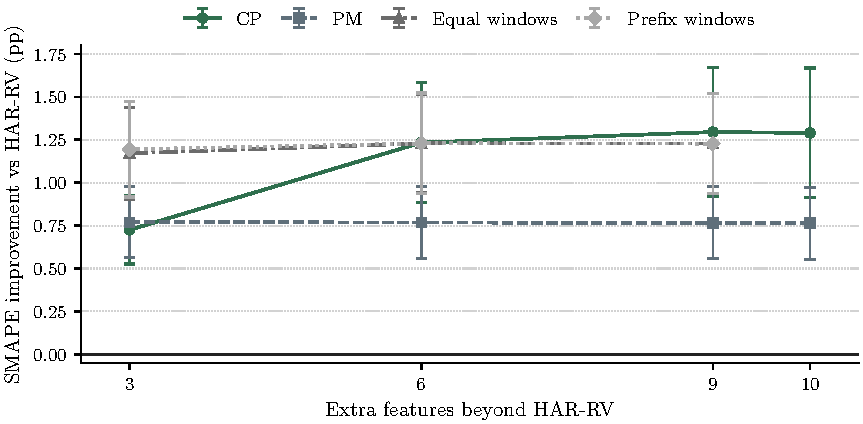
\includegraphics[width=0.82\textwidth]{paper_assets/figures/Section_5_fig_4_feature_count_curve.pdf}
\captionof{figure}{Feature-count curve for ordered and non-ordered lag constructions. Positive values indicate lower SMAPE than HAR-RV.}
\label{fig:feature_count_curve}
\end{center}}

\noindent
Figure~\ref{fig:feature_count_curve} reinforces this interpretation. CP improves sharply between three and six extra features and then flattens, while PM is essentially flat across feature counts. Equal-window and prefix-window controls also improve on HAR-RV, which weakens any claim that primality alone drives the result. The more defensible interpretation is that CP is a compact way to encode useful short-run ordering information.

{\renewcommand{\thefigure}{5}
\begin{center}
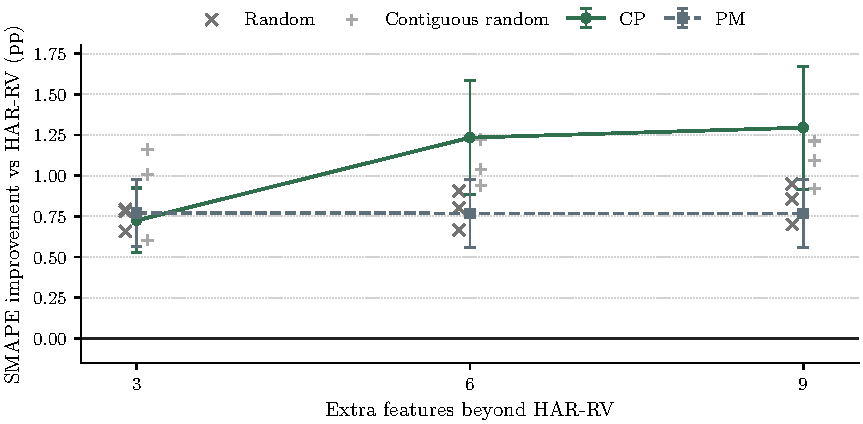
\includegraphics[width=0.82\textwidth]{paper_assets/figures/Section_5_fig_5_random_controls.pdf}
\captionof{figure}{Matched random controls by feature count. Random points show the three tested seeds for RAND and CRS. Positive values indicate lower SMAPE than HAR-RV.}
\label{fig:random_controls}
\end{center}}

\noindent
Figure~\ref{fig:random_controls} compares PM and CP with matched random feature sets. PM is not clearly separated from random controls, especially once the number of added features is fixed. CP is more robust: at six and nine added features it exceeds all sampled RAND and CRS controls. This supports the claim that CP captures a repeatable ordering effect rather than merely benefiting from arbitrary feature enrichment.

\clearpage

{\renewcommand{\thetable}{4}
\begin{center}
\captionof{table}{Driver checks from the robust ablation run. Positive $\Delta$SMAPE indicates lower SMAPE than HAR-RV.}
\label{tab:driver_checks}
\footnotesize
\renewcommand{\arraystretch}{1.12}
\setlength{\tabcolsep}{4pt}
\resizebox{0.98\textwidth}{!}{\input{../final_paper/assets/tables_journal/table_section5_drivers.tex}}

\vspace{0.1cm}
\footnotesize \parbox{0.92\textwidth}{\textit{Notes:} Random-control rows average the three tested seeds. External baselines are interpreted using paired timestamp comparisons against HAR-RV. HAR-TCJ has a shorter aligned sample in raw levels, so the paired $\Delta$SMAPE column is the relevant comparison.}
\end{center}}

\noindent
Table~\ref{tab:driver_checks} separates the main assumptions. Composite and non-coprime modulo controls are nearly identical to PM at matched feature counts, so the prime-modulo construction is not empirically distinguished by primality alone. Local ordered segmentation is more important: CP is stronger than PM and remains competitive against equal, prefix, shifted, and random local controls. EWMA and GARCH(1,1) perform poorly in this intraday realized-volatility setting. HARQ is weakly positive, and HAR-TCJ is not a clear improvement once evaluated on paired timestamps. The robust ablation evidence therefore supports a narrower claim: the strongest contribution is CP's compact ordered local segmentation, not every aspect of the prime-modulo construction.

\subsection{Statistical Significance by Asset Groups}

\noindent
The final question is where the gains are strongest. The broad pattern is that ordered features help most in large, liquid US equity exposures, remain positive but less precise in fixed income and international equity, and add little in commodities and metals.

{\renewcommand{\thefigure}{6}
\begin{center}

\includegraphics[width=0.88\textwidth]{paper_assets/figures/Section_6_fig_7_asset_groups.pdf}
\captionof{figure}{Average SMAPE improvement relative to HAR-RV by asset group.}
\label{fig:asset_groups}
\end{center}}

\clearpage

{\renewcommand{\thetable}{5}
\begin{center}
\captionof{table}{Group-level performance and significance by asset class.}
\label{tab:groups}
\small
\renewcommand{\arraystretch}{1.15}
\setlength{\tabcolsep}{8pt}
\resizebox{0.88\textwidth}{!}{\begin{tabular}{@{}lccc@{}}
\toprule
Asset Group & $\Delta \mathrm{SMAPE}$ (pp) & Asset Win Rate (\%) & Fisher Combined $p$-value \\
\midrule
\multicolumn{4}{@{}l}{\textit{Panel A. Prime Modulo (PM)}} \\
US Mega Tech & 1.26 $\pm$ 0.13 & 100\% & $6.11 \times 10^{-33}$ \\
Broad US Equity & 1.51 $\pm$ 0.10 & 100\% & $6.30 \times 10^{-19}$ \\
International Equity & 0.13 $\pm$ 0.13 & 100\% & $< 10^{-300}$ \\
Commodities/Metals & -0.04 & 0\% & $9.75 \times 10^{-12}$ \\
Fixed Income & 0.31 $\pm$ 0.24 & 100\% & $< 10^{-300}$ \\
\addlinespace
\multicolumn{4}{@{}l}{\textit{Panel B. Contiguous Prime (CP)}} \\
US Mega Tech & 1.79 $\pm$ 0.25 & 100\% & $< 10^{-300}$ \\
Broad US Equity & 2.99 $\pm$ 0.07 & 100\% & $< 10^{-300}$ \\
International Equity & 0.16 $\pm$ 0.34 & 50\% & $< 10^{-300}$ \\
Commodities/Metals & 0.04 & 100\% & $< 10^{-300}$ \\
Fixed Income & 0.59 $\pm$ 0.56 & 100\% & $< 10^{-300}$ \\
\bottomrule
\end{tabular}
}

\vspace{0.1cm}
\footnotesize \parbox{0.92\textwidth}{\textit{Notes:} Positive $\Delta \mathrm{SMAPE}$ indicates lower SMAPE than HAR-RV. Asset Win Rate is the share of assets in each group with positive $\Delta \mathrm{SMAPE}$ relative to HAR-RV. Fisher combined $p$-values aggregate per-asset Diebold--Mariano tests based on absolute-error loss. Values below machine precision are reported as $< 10^{-300}$. Standard errors are unavailable for single-asset groups.}
\end{center}}

\noindent
Figure~\ref{fig:asset_groups} and Table~\ref{tab:groups} make the cross-sectional pattern explicit. The largest gains appear in Broad US Equity and US Mega Tech, where both PM and CP improve on every asset and where CP delivers the largest group-level gains. Fixed Income remains positive but is estimated less precisely, while International Equity is positive on average with wider dispersion. Commodities and Metals are essentially flat, with PM slightly negative and CP only marginally positive.

\noindent
This cross-group pattern is economically coherent. The strongest gains arise in deep, liquid equity exposures where intraday volatility clustering is persistent and ordered lag structure is likely to be informative. Markets that are more exposed to exogenous jumps or thinner intraday participation show much weaker benefits, which suggests that the value of the prime-based extensions depends on the extent to which short-run order carries stable information.


\section{Future Improvements}

\noindent
The present evidence supports a deliberately narrow conclusion: on the ten-asset 5-minute intraday panel, the prime-based extensions improve average forecasting accuracy relative to the HAR-RV baseline, with the strongest and most robust gains coming from CP. The ablations suggest that local ordered segmentation is more important empirically than primality by itself. The appendix daily mirror shows that this advantage does not automatically transfer to daily sampling. Future work should therefore focus less on adding new model names and more on clarifying when ordered lag structure is statistically and economically reliable.

\noindent
A first improvement is to broaden the loss functions used for evaluation. SMAPE, RMSE, MAE, MedAE, and Directional Accuracy cover scale-normalized error, tail-sensitive squared error, absolute error, median robustness, and directional movement. For volatility forecasts, however, a QLIKE-style loss would be a useful addition because it is commonly used for volatility forecast comparison and is less tied to the scale issues of percentage errors \cite{patton2011}. Reporting out-of-sample $R^2$ relative to HAR-RV would also make the magnitude of improvement easier to interpret.

\noindent
A second improvement is to strengthen the inference layer. The current paper uses Newey--West Diebold--Mariano tests and Fisher combined $p$-values, but these tools should be complemented by block-bootstrap confidence intervals for $\Delta$SMAPE and by multiple-testing adjustments across assets, regimes, and model comparisons \cite{politis1994}. If more model variants are reported in future drafts, a model confidence set or a reality-check style procedure would help distinguish genuine predictive improvement from data snooping \cite{hansen2011,white2000}.

\noindent
A third improvement is to make robustness conditional rather than only aggregate. The current regime and asset-group results already point in this direction: prime-based ordering appears more useful in liquid US equity exposures than in commodities, metals, or more jump-driven markets. Future work should test this directly through regime-specific significance tests, separate analyses around market stress periods, and stability checks across alternative intraday windows.

\noindent
Finally, the empirical design should remain fixed while the paper is finalized. The current draft should not change ticker lists, sampling frequency, date range, warmup length, or headline model set unless all sections are regenerated under the same specification. This constraint is important because the paper's main contribution is comparative: the reader should be able to trace each table and figure back to one consistent evaluation panel.

\newpage
\appendix
\renewcommand{\thesection}{Appendix \Alph{section}}

\section{Daily Mirror of Overall Accuracy}

{\renewcommand{\thetable}{1B}
\begin{center}
\captionof{table}{Overall forecasting performance at the daily horizon.}
\label{tab:overall_daily}
\small
\renewcommand{\arraystretch}{1.15}
\setlength{\tabcolsep}{6pt}
\resizebox{0.98\textwidth}{!}{\begin{tabular}{@{}lccccc@{}}
\toprule
Model & SMAPE (\%) & \shortstack{RMSE\\$(\times 10^{-3})$} & \shortstack{MAE\\$(\times 10^{-3})$} & \shortstack{MedAE\\$(\times 10^{-3})$} & \shortstack{Directional\\Accuracy (\%)} \\
\midrule
HAR-RV & \textbf{36.45 $\pm$ 2.46} & \textbf{7.515 $\pm$ 1.002} & \textbf{4.467 $\pm$ 0.527} & \textbf{3.069 $\pm$ 0.354} & \textbf{70.06 $\pm$ 0.69} \\
Prime Modulo (PM) & 37.64 $\pm$ 2.37 & 7.649 $\pm$ 1.014 & 4.640 $\pm$ 0.560 & 3.114 $\pm$ 0.366 & 68.69 $\pm$ 0.89 \\
Contiguous Prime (CP) & 37.88 $\pm$ 2.40 & 7.744 $\pm$ 1.016 & 4.705 $\pm$ 0.569 & 3.121 $\pm$ 0.369 & 69.35 $\pm$ 0.85 \\
\bottomrule
\end{tabular}
}

\vspace{0.1cm}
\footnotesize \parbox{0.92\textwidth}{\textit{Notes:} Lower values are better except for Directional Accuracy. Entries report the cross-sectional mean with standard errors across assets. Error columns are rescaled for readability. Each asset contributes roughly 396 aligned daily observations. Bold marks the best value in each column.}
\end{center}}

\noindent
Table~\ref{tab:overall_daily} is included as a supporting appendix result rather than a main-text finding. On this daily sample, HAR-RV has the lowest average SMAPE, RMSE, MAE, and MedAE, while PM and CP do not preserve the intraday ordering seen in Table~\ref{tab:overall_intraday}. The daily mirror therefore places a clear boundary on the main empirical claim of the paper: the present advantage of the prime-based extensions is concentrated at the intraday horizon rather than being a uniform improvement across sampling frequencies.

\section{Empirical Design}

\noindent
The main empirical panel contains ten liquid assets: AAPL, AMZN, GOOGL, SPY, QQQ, EEM, FXI, GLD, HYG, and TLT. These assets were chosen to cover large-cap US technology, broad US equity exposure, international equity, commodities and metals, and fixed income. The main evaluation uses cleaned 5-minute intraday data. After feature construction, alignment, and warmup, each asset contributes roughly 36,747 evaluation observations.

\noindent
The headline model set is fixed to HAR-RV, PM, and CP. This restriction is intentional. The paper's central claim is not that every engineered variant is useful, but that order-aware prime-based features can improve the HAR-RV baseline under a common data split and evaluation protocol. HAR-RV is therefore the benchmark in every main-text comparison, PM is the direct modular-equivalence extension, and CP is the contiguous prime extension.

\noindent
All reported main-text metrics are first computed separately for each asset and are then summarized across assets. This avoids letting the most densely represented or easiest-to-predict asset dominate the aggregate result. Time-series plots use the cross-sectional average prediction series only for visual clarity; their reported summary statistics are still computed from the underlying full-resolution forecast errors.

\section{Robust Ablation Details}

\noindent
This appendix reports the full robust Section 5 grids. Each entry is a paired comparison against HAR-RV unless otherwise noted. Positive $\Delta$SMAPE means that the candidate model has lower SMAPE than HAR-RV on the aligned evaluation timestamps.

\clearpage

{\renewcommand{\thetable}{C1}
\begin{center}
\captionof{table}{Feature-count curve details. Positive $\Delta$SMAPE indicates lower SMAPE than HAR-RV.}
\label{tab:appendix_feature_count}
\scriptsize
\renewcommand{\arraystretch}{1.08}
\resizebox{0.86\textwidth}{!}{\begin{tabular}{@{}lccccc@{}}
\toprule
Model & Family & Features & $\Delta$SMAPE & SE & Win Rate (\%) \\
\midrule
CP-FC3 & CP & 3 & 0.73 & 0.20 & 44.8 \\
CP-FC6 & CP & 6 & 1.23 & 0.35 & 45.4 \\
CP-FC9 & CP & 9 & 1.30 & 0.38 & 45.3 \\
EQWIN-FC3 & Equal & 3 & 1.17 & 0.27 & 45.7 \\
EQWIN-FC6 & Equal & 6 & 1.23 & 0.29 & 45.8 \\
EQWIN-FC9 & Equal & 9 & 1.23 & 0.29 & 45.8 \\
PM-FC3 & PM & 3 & 0.77 & 0.21 & 43.8 \\
PM-FC6 & PM & 6 & 0.77 & 0.21 & 43.9 \\
PM-FC9 & PM & 9 & 0.77 & 0.21 & 44.0 \\
PREFIX-FC3 & Prefix & 3 & 1.19 & 0.28 & 45.7 \\
PREFIX-FC6 & Prefix & 6 & 1.23 & 0.29 & 45.9 \\
PREFIX-FC9 & Prefix & 9 & 1.23 & 0.29 & 45.9 \\
CP & CP & 10 & 1.29 & 0.38 & 45.3 \\
PM & PM & 10 & 0.76 & 0.21 & 44.0 \\
\bottomrule
\end{tabular}
}
\end{center}}

\noindent
Table~\ref{tab:appendix_feature_count} shows that PM is nearly unchanged as additional modulo features are added. CP improves from three to six features and then flattens, while equal-window and prefix-window controls remain close to CP.

{\renewcommand{\thetable}{C2}
\begin{center}
\captionof{table}{Contiguous-window controls. Positive $\Delta$SMAPE indicates lower SMAPE than HAR-RV.}
\label{tab:appendix_contiguous}
\scriptsize
\renewcommand{\arraystretch}{1.08}
\resizebox{0.90\textwidth}{!}{\input{../final_paper/assets/tables_journal/table_appendix_c2_contiguous.tex}}
\end{center}}

\noindent
Table~\ref{tab:appendix_contiguous} shows that shifted contiguous controls remain positive, but they are weaker than the strongest CP and prefix-window specifications. This supports the importance of local ordering while keeping the exact CP construction as one compact implementation.

\clearpage

{\renewcommand{\thetable}{C3}
\begin{center}
\captionof{table}{Prime and non-prime modulo controls. Positive $\Delta$SMAPE indicates lower SMAPE than HAR-RV.}
\label{tab:appendix_prime_nonprime}
\scriptsize
\renewcommand{\arraystretch}{1.08}
\resizebox{0.84\textwidth}{!}{\begin{tabular}{@{}lccccc@{}}
\toprule
Model & Family & Features & $\Delta$SMAPE & SE & Win Rate (\%) \\
\midrule
COMP-COPRIME-FC6 & Composite & 6 & 0.77 & 0.21 & 43.9 \\
COMP-COPRIME-FC9 & Composite & 9 & 0.77 & 0.21 & 43.9 \\
COMP-NONCOPRIME-FC6 & Non-coprime & 6 & 0.76 & 0.21 & 43.8 \\
COMP-NONCOPRIME-FC9 & Non-coprime & 9 & 0.76 & 0.21 & 44.0 \\
PM-FC3 & PM & 3 & 0.77 & 0.21 & 43.8 \\
PM-FC6 & PM & 6 & 0.77 & 0.21 & 43.9 \\
PM-FC9 & PM & 9 & 0.77 & 0.21 & 44.0 \\
\bottomrule
\end{tabular}
}
\end{center}}

\noindent
Table~\ref{tab:appendix_prime_nonprime} shows that prime, composite, and non-coprime modulo constructions produce very similar paired improvements at matched feature counts. The empirical evidence therefore does not isolate primality as the main driver of the PM result.

\clearpage

{\renewcommand{\thetable}{C4}
\begin{center}
\captionof{table}{Matched random controls. Positive $\Delta$SMAPE indicates lower SMAPE than HAR-RV.}
\label{tab:appendix_random}
\scriptsize
\renewcommand{\arraystretch}{1.08}
\resizebox{0.88\textwidth}{!}{\begin{tabular}{@{}lccccc@{}}
\toprule
Model & Family & Features & $\Delta$SMAPE & SE & Win Rate (\%) \\
\midrule
CP-FC3 & CP & 3 & 0.73 & 0.20 & 44.8 \\
CP-FC6 & CP & 6 & 1.23 & 0.35 & 45.4 \\
CP-FC9 & CP & 9 & 1.30 & 0.38 & 45.3 \\
CRS-FC3-S0 & CRS & 3 & 1.16 & 0.26 & 46.2 \\
CRS-FC3-S1 & CRS & 3 & 0.60 & 0.17 & 44.7 \\
CRS-FC3-S2 & CRS & 3 & 1.01 & 0.24 & 45.5 \\
CRS-FC6-S0 & CRS & 6 & 1.22 & 0.28 & 45.7 \\
CRS-FC6-S1 & CRS & 6 & 0.94 & 0.24 & 45.5 \\
CRS-FC6-S2 & CRS & 6 & 1.04 & 0.25 & 45.6 \\
CRS-FC9-S0 & CRS & 9 & 1.21 & 0.28 & 45.8 \\
CRS-FC9-S1 & CRS & 9 & 0.92 & 0.24 & 45.3 \\
CRS-FC9-S2 & CRS & 9 & 1.09 & 0.26 & 45.4 \\
PM-FC3 & PM & 3 & 0.77 & 0.21 & 43.8 \\
PM-FC6 & PM & 6 & 0.77 & 0.21 & 43.9 \\
PM-FC9 & PM & 9 & 0.77 & 0.21 & 44.0 \\
RAND-FC3-S0 & RAND & 3 & 0.66 & 0.19 & 43.7 \\
RAND-FC3-S1 & RAND & 3 & 0.79 & 0.21 & 44.2 \\
RAND-FC3-S2 & RAND & 3 & 0.78 & 0.20 & 44.5 \\
RAND-FC6-S0 & RAND & 6 & 0.67 & 0.19 & 44.0 \\
RAND-FC6-S1 & RAND & 6 & 0.80 & 0.22 & 44.2 \\
RAND-FC6-S2 & RAND & 6 & 0.91 & 0.23 & 45.0 \\
RAND-FC9-S0 & RAND & 9 & 0.70 & 0.20 & 44.1 \\
RAND-FC9-S1 & RAND & 9 & 0.86 & 0.23 & 44.5 \\
RAND-FC9-S2 & RAND & 9 & 0.95 & 0.24 & 45.3 \\
\bottomrule
\end{tabular}
}
\end{center}}

\noindent
Table~\ref{tab:appendix_random} reports the individual random-control seeds. CP at six and nine features is above all tested RAND and CRS controls. PM is not similarly separated from random controls.

{\renewcommand{\thetable}{C5}
\begin{center}
\captionof{table}{External baseline checks. Positive $\Delta$SMAPE indicates lower SMAPE than HAR-RV on paired timestamps.}
\label{tab:appendix_external}
\scriptsize
\renewcommand{\arraystretch}{1.08}
\resizebox{0.62\textwidth}{!}{\begin{tabular}{@{}lccc@{}}
\toprule
Model & $\Delta$SMAPE vs HAR-RV (pp) & Timestamp Win Rate (\%) & Assets \\
\midrule
HARQ & 0.35 $\pm$ 0.19 & 44.8 & 10 \\
HAR-TCJ & 0.12 $\pm$ 0.59 & 47.5 & 10 \\
EWMA & -10.77 $\pm$ 1.22 & 28.2 & 10 \\
GARCH11 & -16.88 $\pm$ 2.32 & 22.1 & 10 \\
\bottomrule
\end{tabular}
}
\end{center}}

\noindent
Table~\ref{tab:appendix_external} shows that EWMA and GARCH(1,1) are poor fits for this 5-minute realized-volatility target. HARQ is only mildly positive. HAR-TCJ has a much lower raw SMAPE level on its own aligned sample, but the paired comparison against HAR-RV is small and noisy, so it is not treated as a main-text competitor.

\clearpage

\section{Metric Definitions and Inference}

\noindent
Let $y_{i,t}$ denote the realized volatility for asset $i$ at evaluation time $t$, and let $\hat{y}^{\,m}_{i,t}$ denote the forecast from model $m$. Define the forecast error $e^{\,m}_{i,t} = y_{i,t} - \hat{y}^{\,m}_{i,t}$. All main-text tables first compute metrics at the asset level and then average those asset-level quantities across the cross-section.

\vspace{0.15cm}
\noindent \textbf{Forecast metrics.}
For an asset with $T_i$ aligned evaluation observations, the reported metrics are
\begin{align*}
\mathrm{SMAPE}^{\,m}_i &= \frac{200}{T_i}\sum_{t=1}^{T_i}\frac{|y_{i,t}-\hat{y}^{\,m}_{i,t}|}{|y_{i,t}|+|\hat{y}^{\,m}_{i,t}|},\\
\mathrm{RMSE}^{\,m}_i &= \sqrt{\frac{1}{T_i}\sum_{t=1}^{T_i}\left(e^{\,m}_{i,t}\right)^2},\\
\mathrm{MAE}^{\,m}_i &= \frac{1}{T_i}\sum_{t=1}^{T_i}\left|e^{\,m}_{i,t}\right|,\\
\mathrm{MedAE}^{\,m}_i &= \mathrm{median}_{1 \leq t \leq T_i}\left|e^{\,m}_{i,t}\right|.
\end{align*}
Directional Accuracy is computed from the sign of the realized next-step change relative to the sign implied by the forecast:
\begin{align*}
\mathrm{DA}^{\,m}_i
= \frac{100}{T_i-1}\sum_{t=2}^{T_i}
\mathbf{1}\!\left\{
\mathrm{sign}(y_{i,t}-y_{i,t-1})
=
\mathrm{sign}(\hat{y}^{\,m}_{i,t}-y_{i,t-1})
\right\}.
\end{align*}

\vspace{0.15cm}
\noindent \textbf{Cross-sectional aggregation.}
If $M_i^{\,m}$ denotes any one of the asset-level metrics above, the tables report
\begin{align*}
\bar{M}^{\,m} &= \frac{1}{N}\sum_{i=1}^{N} M_i^{\,m},\\
\mathrm{SE}\!\left(\bar{M}^{\,m}\right) &= \frac{s(M_1^{\,m},\ldots,M_N^{\,m})}{\sqrt{N}},
\end{align*}
where $N$ is the number of assets and $s(\cdot)$ is the sample standard deviation across assets.

\vspace{0.15cm}
\noindent \textbf{Advantage measures used in Figures 3 and 6 and in Table 5.}
For the timestamp-level advantage plot, we define
\begin{align*}
\delta_t^{\,m}
=
\mathrm{SMAPE}_{\mathrm{HAR},t}
-
\mathrm{SMAPE}_{m,t},
\end{align*}
so positive values indicate that model $m$ improves on HAR-RV at time $t$. The summary statistics in Figure~\ref{fig:error_advantage} are then based on the full-resolution sequence $\{\delta_t^{\,m}\}$:
\begin{align*}
\overline{\delta}^{\,m} &= \frac{1}{T}\sum_{t=1}^{T}\delta_t^{\,m},\\
\mathrm{WinRate}^{\,m}_{\mathrm{time}} &= \frac{100}{T}\sum_{t=1}^{T}\mathbf{1}\{\delta_t^{\,m}>0\},\\
\mathrm{CLD}^{\,m} &= \sum_{t=1}^{T}\delta_t^{\,m}.
\end{align*}
For the asset-group analysis, the relevant object is the asset-level improvement
\begin{align*}
\Delta \mathrm{SMAPE}^{\,m}_i
=
\mathrm{SMAPE}^{\,\mathrm{HAR}}_i
-
\mathrm{SMAPE}^{\,m}_i,
\end{align*}
which is averaged within each group $g$ as
\begin{align*}
\overline{\Delta \mathrm{SMAPE}}^{\,m}_g
=
\frac{1}{N_g}\sum_{i \in g}\Delta \mathrm{SMAPE}^{\,m}_i,
\qquad
\mathrm{WinRate}^{\,m}_g
=
\frac{100}{N_g}\sum_{i \in g}\mathbf{1}\{\Delta \mathrm{SMAPE}^{\,m}_i>0\}.
\end{align*}
Accordingly, the win rate in Figure~\ref{fig:error_advantage} is a timestamp-level quantity, whereas the win rates in Table~\ref{tab:groups} are asset-level quantities.

\vspace{0.15cm}
\noindent \textbf{Diebold--Mariano and Fisher combined inference.}
For a given loss function $L(\cdot)$, the asset-level Diebold--Mariano test is built from the loss differential
\begin{align*}
d^{\,m}_{i,t}
=
L\!\left(e^{\,\mathrm{HAR}}_{i,t}\right)
-
L\!\left(e^{\,m}_{i,t}\right),
\end{align*}
with statistic
\begin{align*}
\mathrm{DM}^{\,m}_i
=
\frac{\bar{d}^{\,m}_i}{\sqrt{\widehat{\mathrm{Var}}_{\mathrm{NW}}(\bar{d}^{\,m}_i)}}.
\end{align*}
Figure~\ref{fig:error_advantage} applies this logic to the timestamp-level SMAPE differential, while Table~\ref{tab:groups} combines per-asset Diebold--Mariano $p$-values based on absolute-error loss \cite{diebold1995}. If $\{p^{\,m}_{i,g}\}_{i \in g}$ are the valid per-asset $p$-values for group $g$, the Fisher combined statistic is
\begin{align*}
X^{\,m}_g &= -2\sum_{i \in g}\log p^{\,m}_{i,g},\\
p^{\,m,\mathrm{Fisher}}_g &= 1 - F_{\chi^2_{2N_g}}\!\left(X^{\,m}_g\right),
\end{align*}
where $F_{\chi^2_{2N_g}}$ is the chi-squared cumulative distribution function with $2N_g$ degrees of freedom.


\begin{thebibliography}{9}

\bibitem{corsi2009}
F. Corsi.
\newblock A simple approximate long-memory model of realized volatility.
\newblock \textit{Journal of Financial Econometrics}, 7(2):174--196, 2009.
\newblock doi: 10.1093/jjfinec/nbp001.

\bibitem{diebold1995}
F. X. Diebold and R. S. Mariano.
\newblock Comparing predictive accuracy.
\newblock \textit{Journal of Business \& Economic Statistics}, 13(3):253--263, 1995.
\newblock doi: 10.1080/07350015.1995.10524599.

\bibitem{hansen2011}
P. R. Hansen, A. Lunde, and J. M. Nason.
\newblock The model confidence set.
\newblock \textit{Econometrica}, 79(2):453--497, 2011.
\newblock doi: 10.3982/ECTA5771.

\bibitem{patton2011}
A. J. Patton.
\newblock Volatility forecast comparison using imperfect volatility proxies.
\newblock \textit{Journal of Econometrics}, 160(1):246--256, 2011.
\newblock doi: 10.1016/j.jeconom.2010.03.034.

\bibitem{politis1994}
D. N. Politis and J. P. Romano.
\newblock The stationary bootstrap.
\newblock \textit{Journal of the American Statistical Association}, 89(428):1303--1313, 1994.
\newblock doi: 10.1080/01621459.1994.10476870.

\bibitem{white2000}
H. White.
\newblock A reality check for data snooping.
\newblock \textit{Econometrica}, 68(5):1097--1126, 2000.
\newblock doi: 10.1111/1468-0262.00152.


\end{thebibliography}

\end{document}
